% Title:       14. Bayerischer \TeX{}-Stammtisch in Regensburg
% Author:      Leo Arnold (@leoarnold)
% URL:         https://github.com/BayTeX/2016Regensburg
% License:     CC BY 4.0 - http://creativecommons.org/licenses/by/4.0/

\documentclass[ngerman]{dtk} 

\ifluatex
  \usepackage[utf8]{luainputenc}
\else
  \usepackage[utf8]{inputenc}
\fi

\usepackage{graphicx, tabularx}

\addbibresource{baytex2016-bericht.bib}

\title{14. Bayerischer \TeX{}-Stammtisch in Regensburg} 
\Author{Leo}{Arnold}{\Email{baytex@leoarnold.de}}

\begin{document}
\maketitle
\markboth{14. Bay\TeX{} 2016}{14. Bay\TeX{} 2016}

\begin{abstract}
Die vielleicht erste \TeX{}-Konferenz in der Oberpfalz,
ein engagiertes junges Organisationsteam und warum es fast nicht dazu gekommen wäre \ldots
\end{abstract} 

\section{Was bisher geschah}
Einmal im Jahr schalten sich die Stammtische in Erlangen und München zusammen,
um gemeinsam eine kleine Konferenz mit großem Mehrwert auf die Beine zu stellen
-- oder wie es ein Vorstandsmitglied einmal überspitzt zusammenfasste:
\begin{quote}
\itshape \enquote{Die Bayern brauchen halt immer eine Extrawurst.}
\end{quote}
Das ist natürlich zu kurz gegriffen. Die Bay\TeX{} freut sich über alle Teilnehmenden,
unbesehen ihrer Herkunft, und ist auch regional nicht auf die Landesgrenzen des Freistaates beschränkt.
So wurde die Veranstaltung von 2006 bis 2009 vom Stammtisch Ulm mit organisiert und fand auch zweimal dort statt.

Mittlerweile sind die Stammtische auf ihren harten Kern geschrumpft und es fällt schwer,
neue Teilnehmer für die Stammtische und die Vereinsmitgliedschaft zu begeistern.
Um so wichtiger scheint es, die verbliebenen Enthusiasten überregional zu vernetzen
und durch kleine informelle Veranstaltungen wie die Bay\TeX{} potentiellen Interessenten die Scheu vor der Teilnahme zu nehmen,
sowie die Sichtbarkeit der Anwendergruppen zu erhöhen.

Es war also an der Zeit, unsere ausgetretenen Pfade zu verlassen und nach elf Jahren Rotation
zwischen Erlangen-Nürnberg, München und Ulm endlich neues Land zu erkunden.
So haben wir uns sehr gefreut, als uns Doris Behrendt 2014 ins unterfränkische Marktbreit eingeladen hat.
Dort überzeugten sich auch Peter Zimmermann und sein Team von der Veranstaltung und luden uns im Folgejahr nach Eichstätt ein.
Doch da endete unsere Glückssträhne der Einladungen auch wieder \ldots oder doch nicht?

\section{Aufbruch ins Ungewisse}
Auch wenn es der CSU nicht bewusst zu sein scheint: Bayern ist ein Vielvölkerstaat.
Neben Bayern und Franken wohnen hier auch Schwaben und Oberpfälzer.
Ein kurzer Blick in die Chroniken förderte die erschütternde Erkenntnis,
dass weder die Bay\TeX{}, noch eine Tagung der Dante je in der Oberpfalz stattgefunden hatten.
So fasste ich den Entschluss, die Veranstaltung nach Regensburg zu bringen.

\subsection{Ungefragt angeschrieben}
Der einzige Knackpunkt bei der Organisation einer Bay\TeX{} ist es, einen Raum zu finden.
Insbesondere, wenn man sich einen Veranstaltungsort in den Kopf gesetzt hat, an dem man niemanden kennt.
Schlaue Menschen hätten an dieser Stelle das DTK-Archiv nach dem Begriff \enquote{Regensburg} durchsucht,
aber mich führte auch der Umweg über die Weiten des Internets zu Marei Peischl,
die seit fast fünf Jahren mit großem Einsatz Einführungskurse in \LaTeX{} an der Uni Regensburg abhält.
So schickte ich eine vorsichtige Anfrage, ob sie mir weiterhelfen könne,
und fiel ein paar Tage später fast vom Bürostuhl, als sie mir antwortete,
dass sie schon ein Organisationsteam zusammengestellt und einen Raum gefunden hatte.
Schließlich gab es in Regensburg noch keinen \TeX{}-Stammtisch und die Konferenz
könnte dazu führen, ihre Studenten und andere interessierte Regensburger
endlich mal an einen Tisch zu bringen.
Die Rückmeldung aus Erlangen und München war eindeutig: Regensburg, wir kommen!
So schnell hatten wir noch nie eine Bay\TeX{} koordiniert. Und auch diesmal sollte es anders kommen.

\subsection{Da passiert schon nichts \ldots}
Man könnte meinen, dass diverse akademische Institute ein Interesse daran haben,
\TeX{}-Anwendergruppen zu unterstützen und so eine wichtige kostenfreie
Anlauf- und Beratungsstelle für ihre Studenten zu erhalten.
Leider ist hier die Euphorie gewichen und so treten bürokratische Fragestellungen
in den Vordergrund. An der Uni Regensburg hätte man uns einerseits gerne einen Hörsaal kostenfrei überlassen,
andererseits gab es in der Vergangenheit mehrere kostenintensive Zwischenfälle.
Per Gesetz haftet dafür natürlich der Verursacher.
Der ließ sich jedoch nicht ermitteln, weshalb die Kosten auf den jeweiligen Veranstalter - schlussendlich also die Universität - zurück fielen, und so etwas wollte man nicht noch einmal erleben.
So wurden wir aufgefordert, einen Veranstalter zu benennen, der im Fall des Falles die Kosten trägt.

Auf den Veranstalter einer Tagung kommen allerhand rechtliche Auflagen zu.
So muss er unter anderem für Brandschutz und ausreichende Fluchtmöglichkeiten sorgen.
Das ist für die Universität kein Problem,
da sie diese Bedingungen auch sonst regelmäßig prüfen muss.
Für einen externen Veranstalter stellt dies natürlich eine weitere Hürde dar.
Dies ist der Grund, warum Dante e.\,V. noch nie Veranstalter
einer Tagung war, sondern sich stets von lokalen Organisatoren als Vertreter der veranstaltenden Universität einladen lässt.
Wir wollen an dieser Stelle nicht verschweigen, dass durch diesen Kniff auch die Raummiete und das Haftungsrisiko für den Verein entfallen.

Einerseits haben wir noch nie gehört, dass auf einer \TeX{}-Tagung mehr kaputt gegangen ist, als ein paar Kaffeetassen.
Andererseits möchte man keine Privatperson dem Kostenrisiko eines versehentlich ausgelösten Feueralarms o.\,Ä. aussetzen.
Insbesondere dann nicht, wenn diese Person schon die Last auf sich genommen hat, die gesamte Organisation zu übernehmen.

Natürlich ließe sich die Haftungsfrage mit einer Veranstaltungsversicherung für ca. 100 Euro klären.
Und die Vereinskasse von Dante ist prall gefüllt.
Sogar so prall, dass dem Verein immer wieder die Aberkennung
der Gemeinnützigkeit droht.
Doch der Vorstand bezieht hier eine eindeutige Position:
Gerne finanzielle Förderung von Veranstaltungen,
jedoch nicht zur Bezahlung von Raummieten oder Versicherungen.

So fand unser Enthusiasmus ein jähes Ende.
Eine \TeX{}-Tagung, deren Organisationsteam einen Altersschnitt von unter 30 hat, das wäre eine echte Sensation gewesen.
Ich hielt Rücksprache mit befreundeten Eventmanagern.
Sie bestätigten mir die grundsätzliche Haftung des Veranstalters und rieten dringend
zur Versicherung.
Resignation machte sich breit und wir legten die Pläne ad acta.

\subsection{Da passiert doch noch was}
Und plötzlich meldete sich der Stammtisch Erlangen.
Sie hatten aus eigener Initiative das Rechenzentrum der Uni Regensburg kontaktiert
und dort hatte man sich bereit erklärt, das Haftungsrisiko zu übernehmen
und als Veranstalter aufzutreten.
Ein wagemutiger Schritt, wenn man bedenkt, wie heiß es bei Tagungen auch ohne Mitgliederversammlung her gehen kann.
Von Kleinkriegen wie PSTricks gegen TikZ bis zur großen ideologischen Frage,
wie man nur \TeX{}live verwenden kann, wenn der \texttt{tlmgr} bei Lizenzproblemen
auch mal Pakete eigenmächtig wieder vom Rechner löscht.
Man kann wohl von einem Wunder sprechen, dass bei der diesjährigen Bay\TeX{} alle Beteiligten bis auf zahlreiche Insektenstiche unverletzt blieben.

\section{Auf der Hauptbühne}
Zu den Besonderheiten der Bay\TeX{} gehört es wohl, dass das Programm stets prall gefüllt ist.
Die drei Vortragsplätze sind meist schnell vergeben und oft werden es noch mehr.
Auch kurze Beiträge sind immer gern gesehen, denn auf der Bay\TeX{} herrscht
eine rege Interaktionskultur, die jedem Referenten genügend Gelegenheiten eröffnet,
sein Fachwissen in Exkursen zu demonstrieren, und die Zeit dafür nehmen wir uns.
Peter Seitz berichtete uns, dass schon bei der ersten Bay\TeX{} im Jahr 2003
die zwei kurzen Vorträge zu einer angeregten Plenumsdiskussion von vier Stunden ausuferten.

\begin{center}
\begin{tabularx}{\linewidth}{*{2}{>{\centering\arraybackslash}X}}
Klaus Neudecker & Oliver Rath\\
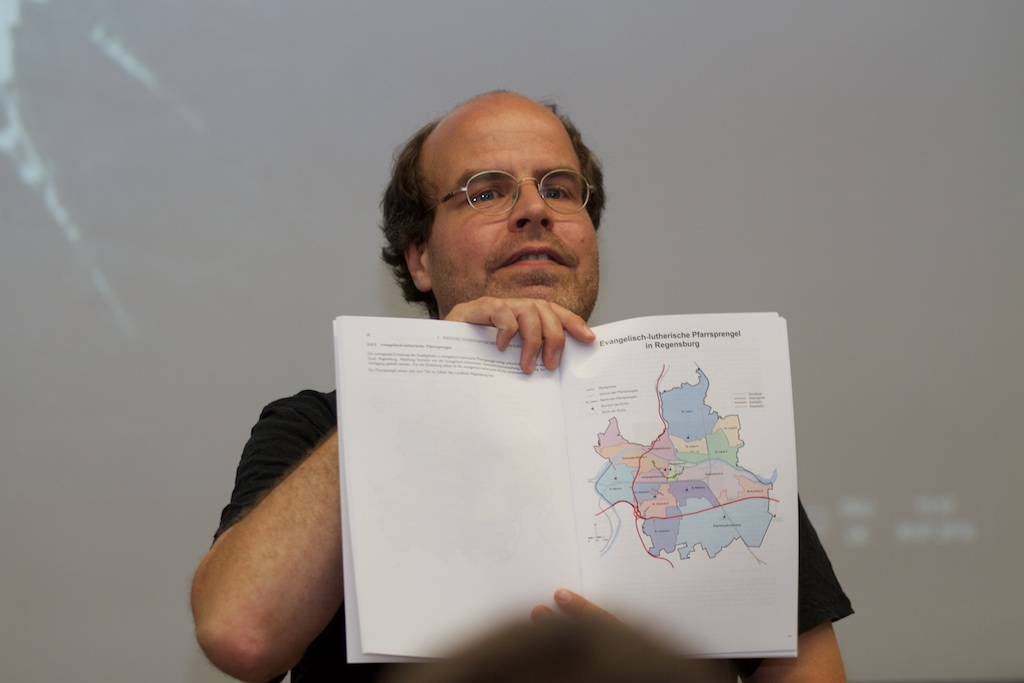
\includegraphics[width=\linewidth]{neudecker.jpg}
& 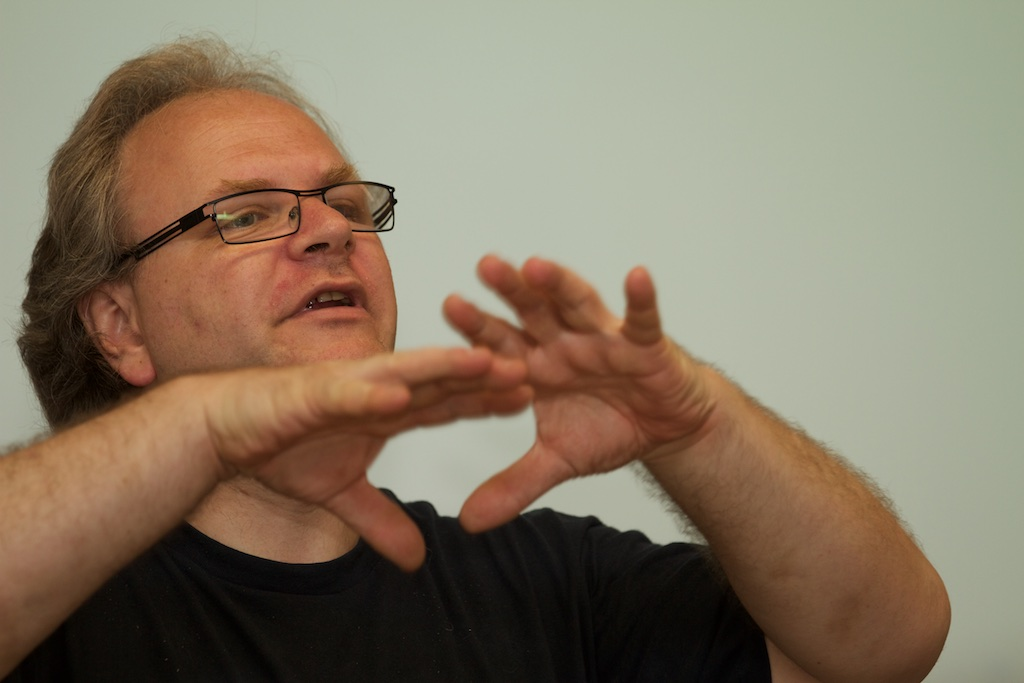
\includegraphics[width=\linewidth]{rath.jpg}
\\[1ex]
Harald König & Bay\TeX{} 2016\\
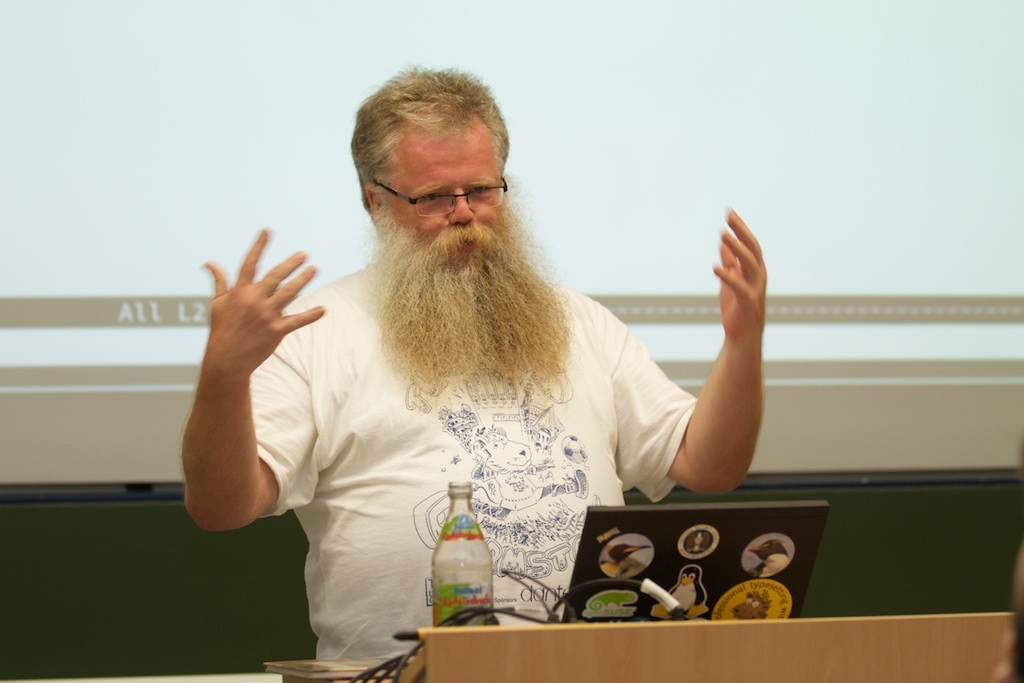
\includegraphics[width=\linewidth]{koenig.jpg}
& 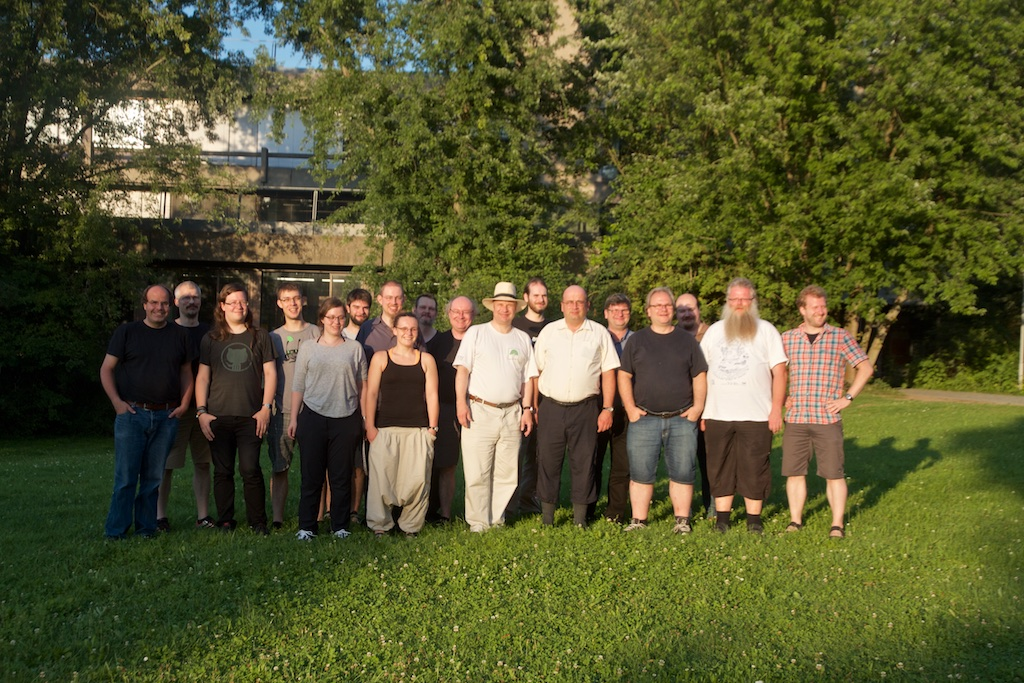
\includegraphics[width=\linewidth]{gruppe.jpg}
\\[1ex]
\multicolumn{2}{c}{(Fotos von Benno Pütz)}
\end{tabularx}
\end{center}

\subsection{\TeX{}nische Einblicke in die Regensburger Stadtverwaltung}
Wenn man \enquote{LaTeX Regensburg} in eine Suchmaschine eingibt,
findet man wohl kaum, wonach man ursprünglich suchen wollte.
Sucht man hingegen \enquote{pdflatex Regensburg},
so findet man unter den ersten Treffern das Regensburger Straßenverzeichnis \cite{strassenverzeichnis}.
Eine deutsche Behörde, die \LaTeX{} verwendet?!
Einen kurzen Postwechsel später konnten wir Klaus Neudecker vom Amt für Stadtentwicklung der Stadt Regensburg als Referenten gewinnen, der uns mit seinem Vortrag über die Arbeit in der Abteilung für Statistik begeisterte.

Wissen Sie, welches Kirchenamt und welche Polizeidienststelle für Ihren Wohnsitz zuständig ist? Kennen Sie den Unterschied zwischen einem Wahlkreis und einem Stimmkreis? Es gibt viele verschiedene Aspekte, nach denen sich eine Stadt gliedern lässt, und jedes Mal entsteht dabei ein anderes Bild. Die Abteilung für Statistik der Stadt Regensburg hat den Auftrag, all diese Gliederungen zu erfassen und den anderen Abteilungen zugänglich zu machen.

In seinem Vortrag erzählte uns Klaus Neudecker wie er zu diesem Zweck eine verwaltungsinterne Weboberfläche entwickelte, auf welcher sich Daten gezielt auswählen und in vielen verschiedenen Formaten exportieren lassen. Insbesondere gibt es dabei die Möglichkeit, die Daten als \LaTeX{}-Quelldokument zu bekommen und damit die zahlreichen Publikationen \cite{regensburg} der Abteilung sachlich korrekt und optisch ansprechend zu gestalten. Viele davon sind bereits kostenlos verfügbar, da sich Klaus Neudecker sehr für Transparenz und \enquote{Open Data} einsetzt.

\subsection{\textsl{Word}los glücklich}
In der Geschäftswelt hat sich \textsl{Word} als de-facto Standard für die Erstellung von Dokumenten durchgesetzt. Als Austauschformat sind DOCX und ODT jedoch eher ungeeignet: das Layout ist nie dasselbe, wenn man das Dokument nicht mit derselben Version desselben Programms öffnet.
Oliver Rath berichtet uns, wie er in einem Unternehmen eine Lösung auf Basis von AsciiDoc implementiert hat.

AsciiDoc ist eine simple Auszeichnungssprache, bei der die spätere Formatierung des Textes durch Sonderzeichen wie in \texttt{'kursiv'} und \texttt{+monospaced+} gekennzeichnet wird.
Im Gegensatz zu Formaten wie MarkDown oder Textile ist AsciiDoc erweiterbar.

Das neue Format wurde von allen Autoren, Technikern und Nicht-Technikern, gut angenommen und sorgt nun für einheitliche Formatierung unabhängig vom verwendeten Editor.
Abgeschlossene Dokumente können unter anderem in die Formate \LaTeX{}, PDF, ODT oder DOCX konvertiert werden.

\subsection{Die Harald XML Picture Show}
Um ein Fotobuch zu erstellen ist die Software der Firma CEWE sehr hilfreich. Allerdings sind ihr auch typographische Grenzen gesetzt und natürlich erhält man kein druckfertiges PDF, da CEWE gerne den Druckauftrag hätte.
Um ein Fotobuch ganz nach seinen eigenen Vorstellungen erzeugen zu können, nahm Harald König das Dateiformat der Software unter die Lupe.
Mit Kreativität und Tüftelei erkannte er in einer großen XML-Datei nach und nach die Werte für Position und Größe seiner Fotos.

In seinem Vortag zeigte uns Harald zunächst, wie man mit Con\TeX{}t eine XML-Datei einlesen kann.
Im ständigen Wechsel zwischen Erläuterungen zur Struktur der CEWE-Daten und den nötigen Con\TeX{}t-Befehlen entstand vor unseren Augen ein Dokument,
das dem Ausgangsmodell von CEWE Schritt für Schritt immer ähnlicher wurde.
Zudem hatte Harald einige Fotobücher von CEWE und aus eigenem Satz mitgebracht,
anhand derer wir die Qualität in direkter Gegenüberstellung vergleichen konnten.

\section{Im Backstage-Bereich}
Für den Gastgeber liegt am Tag der Konferenz der größte Aufwand sicherlich in der Verpflegung der Teilnehmer.
Der Kaffee sollte rechtzeitig zur Pause fertig sein und der Grill muss früh genug angeheizt werden.
Das Regensburger Team verwöhnte die Teilnehmer darüber hinaus zusätzlich mit diversen selbst gebackenen Kuchen zum Kaffee
und selbst gemachten Salaten zu Schnitzel und natürlich Bratwurst.
Die BayTeX entwickelt sich somit auch kulinarisch zu einem Highlight und setzt die Erwartungen hoch für zukünftige Veranstalter.

\section{Danksagung}
Wir möchten uns ausgiebig bei Marei Peischl bedanken, die sich unermüdlich für das Zustandekommen der Konferenz
eingesetzt hat, und ebenso ihrem Team, welches unter ihrer Leitung eine fantastische Tagung organisiert hat,
die wirklich keine Wünsche offen ließ. Weiter danken wir den Referenten, die uns bestens unterhalten haben
deren Vorträge genügend Anregungen für interessante Diskussionen boten.
Wir freuen uns darüber, dass wir Dante e.\,V. auch dieses Jahr wieder zu unseren Sponsoren zählen dürften,
und legen als Dank dafür gerne diesen Bericht vor.
Zum Schluss gilt noch ein besonderer Dank der Universität Regensburg, insbesondere ihrem Rechenzentrum,
welches als Veranstalter schützend die Hand über unsere kleine Konferenz gehalten hat.

\section{Bis nächstes Jahr}
Wir bemühen uns, weiter mit dem kanonischen Wechsel zwischen den Großräumen München und Nürnberg zu brechen.
Gerne nehmen wir Vorschlage für künftige Gastgeber unter \Email{baytex@leoarnold.de} entgegen.

Die Bay\TeX{} freut sich stets über neue Teilnehmer und Referenten.
Für das kommende Jahr planen wir eine Veranstaltung in München,
über die wir im Frühjahr 2017 auf der Mailingliste von Dante e.\,V.
und der Website von Walter Schmidt \cite{cq131a} informieren werden.
Wir würden uns freuen, Sie begrüßen zu dürfen.

\printbibliography

\end{document}